\chapter{MCTDH Theorie}

\section{Einleitung}
Die Entwicklung von Methoden, die eine genaue quantendynamischen Berechnung von mehratomaren Systemen erm"oglichen, stellen die theoretische Chemie und
chemische Physik vor eine wesentliche Herausforderung.
Der MCTDH-Ansatz[16,17paper] spielt eine entscheidende Rolle am Erfolg der Entwicklung quantendynamischer Rechenmethoden.
Mit dem MCTDH-Ansatz konnten Reaktionsraten von Reaktionen mit sechs Atomen wie $H+CH_{4} \rightarrow H_{2} + CH_{3}$ [10-14paper]
und $ O + CH_{4} \rightarrow OH + CH_{3} $ [15paper] berechnet werden.
Des Weiteren konnten Tunnelaufspaltungen und Schwingungszust"ande von Malonaldehyd[18paper] und dem $ H_{5}O^{+}_{2} $-Cluster[7-9paper] berechnet werden.
Sowohl die Schwingungsdynamiken von lichtangeregten Pyrazin [19paper] und von photoionisierten Butatrien [20paper] als auch der Elektronentransfer
aus einem angeregten Zustandes in "Ubergangsmetallen [21,22paper]  konnten mithilfe des MCTDH-Ansatzes untersucht werden.
\\Um molekulare Systeme theoretisch untersuchen zu k"onnen, muss zun"achst die Schr"odingergleichung (SGL) gel"ost werde.
Um die SGL zu l"osen, muss die Wellenfunktion, die das System beschreiben soll, definiert werden.
Generell wird die Wellenfunktion durch das Produkt von mehrdimensionalen zeitabh"angigen Basisfunktionen dargestellt.
Dieser Ansatz der Wellenfunktion wird in der Standardmethode verwendet. [meyer rev 2011]
 Die Basisfunktionen werden in einer eindimensionalen zeitunabh"angigen Basis mit den jeweiligen zeitabh"angigen Koeffizienten entwickelt.
F"ur jeden Freiheitsgrad $f$ des Systems ergeben sich $N$ zeitunabh"angige Basisfunktionen. Somit w"achst die Anzahl der Entwicklungskoeffizienten um $N^{f}$ und
die Standardmethode skaliert exponentielle, sodass nur kleinere Systeme berechenbar sind. [meyer rev 2011]
  \\ Im Unterschied zu der Standardmethode resultiert die Effizienz des MCTDH aus der Doppellayerstruktur der verwendeten Wellenfunktion.
Anstelle die Wellenfunktion in einer zeitunab"angigen Basis zu entwickeln und die Zeitentwicklung durch zeitabh"angige Entwicklungskoeffizienten zu beschreiben,
wird in der MCTDH - Methode die Wellenfunktion als ein Satz von zeitabh"angigen Basisfunktionen dargestellt.
Diese zeitabh"angigen Basisfunktionen werden Einteilchenfunktionen (SPF) genannt und in einer primitiven zeitunabh"angigen Basis dargestellt.
Die Doppellayerstruktur des MCTDHs resultiert aus zwei Entwicklungen mit jeweils zeitabh"angigen Entwicklungskoeffiziente:
Zum einen stellen die Entwicklungskoeffizienten mit den SPFs die korrelierte Wellenfunktion dar und bilden den oberen MCTDH -
Layer und zum anderen k"onnen die SPFs durch die Entwicklungskoeffizienten in der primitiven zeitunabh"angigen Basis entwickelt werden. Diese Entwicklung bildet
den unteren Layer.[Manthe, 2008 multilayer MCTDH approach]
  \\ Die Anzahl der SPFs kann verglichen mit der primitiven Basis signifikant kleiner gew"ahlt werden.
Dennoch ist auch das MCTDH durch eine exponentielle Skalierung limitiert.
Um Korrelationseffekte beschreiben zu k"onnen, sind mindestens zwei SPFs pro Freiheitsgrad notwendig, sodass der numerische Aufwand mit der Anzahl der
Freiheitsgrade $f$ zu $2^f$ skaliert. Aufgrund dieser Skalierung k"onnen Systeme mit maximal 12 - 14 korrelierten Koordinaten [10-15,27,28] behandelt werden.
  \\ Zus"atzliche zu der Doppellayerstruktur k"onnen die Koordinaten in ,,logische`` und physikalische Koordinaten unterschieden werden und
verschiedene physikalischen Koordinaten werden zu einzelne logische Koordinaten kombiniert. Die logischen Koordinaten werden Partikel genannt, sodass
nicht die Anzahl der Freiheitsgrade der limiterende Faktor f"ur die modenkombinierte MCTDH-Rechnung ist,
sondern die Anzahl der Partikel $p$. So konnten Systeme mit 15 - 24 korrelierten Freiheitsgraden [8,9,19,20] und System-Bad-Modelle [31-33] behandelt werden.
Dennoch bleibt das Problem der exponentielle Skalierung von $2^p$ bestehen.
  \\Dieses Problem wird mit dem multilayer (ML)-MCTDH-Ansatz [34] begegnet.
Die SPFs k"onnen selbst als mehrdimensionale Wellenfunktionen dargestellt werden und in anderen SPF entwickelt werden.
Bei drei Layern wird der obere Layer durch die SPF-Basis des herk"ommlichen MCTDHs gebildet.
Diese Basis wird als SPFs des ersten Layers bezeichnet und kann selbst in der SPF-Basis des zweiten Layers entwickelt werden.
Die SPF-Basis des zweiten Layers erweitert das MCTDH um einen weiteren Layer und wird selbst in der primitiven Basis entwickelt, die den unteren Layer bildet.
Durch die rekursive Anwendung der MCTDH - Methode k"onnen weitere Layer zugef"ugt.
Mit der ML-MCTDH Methode sind quantumdynamische Rechnungen von System-Bad Modellen mit bis zu 1000 korrelierten Koordinaten m"oglich,
in denen Elektronentransferprozesse [34-35] untersucht wurden.
 \\Um die MCTDH-Wellenfunktion propagieren zu k"onnen, m"ussen die Matrixelemente des Hamiltonoperators effizient berechnet werden.
So lange der Hamiltonoperator der Summe von Produkten von Einteilchenoperatoren [17] entspricht, stellt die Berechnuung der Matrixelemente kein Probelm dar.
Im Gegensatz zu vielen Modelhamiltonoperatoren k"onnen \textit{ab initio} Potentialenergiefl"achen nicht in dieser Form dargestellt werden.
Durch die Verwendung einer spezifischen zeitabh"angigen Quadratur, die die Matrixelemente allgemeiner Potentiale effizient auswertet, k"onnen
auch Matrixelemente solcher \textit{ab initio} Potentialenergiefl"achen effizient berechnet werden.
Diese Vorgehensweise wird correlation discrete variable representation (CDVR) [40,41] genannt.
 \\Das urspr"ungliche Vorgehen f"ur das CDVR [40] beruht auf ein zeitabh"angiges DVR-Gitter, das direkten Produkten einer SPF-Basisfunktion entspricht.
Somit kann das Standard-CDVR weder f"ur modenkombinierte MCTDH-Rechnungen noch f"ur Berechnungen mit dem ML-MCTDH-Ansatz verwendet werden.
 \\Allerdings konnte ein CDVR , das ohne ein direktes Produktgitter auskommt, in modenkombinierte MCTDH-Rechnungen verwendet werden. [42]
 Der numerische Aufwand des CDVRs h"angt linear von der Anzahl der verwendeten primitiven Gitterpunkten ab, die f"ur die Darstellung der SPFs ben"otigt werden.
In modenkombinierte MCTDH-Rechnungen wird eine gro"se Anzahl an primitiven Gitterpunkten verwendet, sodass modenkombinierte MCTDH-Rechnungen kombiniert mit CDVR-
Auswertung des Potentials ineffizient sind. ML-MCTDH-Rechnungen ben"otigen dagegen keine mehrdimensionalen Gitter, um die SPFs darzustellen, und bieten sich
in Kombination mit dem CDVR an.

\section{Layerstruktur der MCTDH - Wellenfunktion}

Ziel ist es die zeitabh"angige SGL

\begin{equation}
i\dot{\Psi} = H \Psi
\label{Eq:SGL}
\end{equation}

zu l"osen.
  \\Zur L"osung von Gleichung \ref{Eq:SGL} kann die Wellenfunktion $\Psi$ in einer zeitunabh"angigen Basis $\mathcal{X}^{\kappa}_{j}(x_{\kappa})$ entwickelt werden:

 \begin{equation}
 \Psi(x_{1},..., x_{f}, t)=\sum^{N_{1}}_{j_{1}=1} ... \sum^{N_{f}}_{j_{f}=1} A^{1}_{j_{1}, ..., j_{f}}(t)\cdot \mathcal{X}^{(1)}_{j_{1}}(x_{1}) \cdot ... \cdot \mathcal{X}^{(f)}_{j_{f}}(x_{f})
 \label{Eq:Std_wave}
 \end{equation}

Die zeitabh"angigen Koeffizienten $A^{1}_{j_{1}, ..., j_{f}}(t)$ beschreiben die Bewegung der Wellenpakete.
Die Darstellung der Wellenfunktion in Gleichung  \ref{Eq:Std_wave} kann auch als Einfachlayerdarstellung betrachtet werden.
Im Unterschied zu Gleichung \ref{Eq:Std_wave} wird die MCTDH - Wellenfunktion,

 \begin{equation}
 \Psi(x_{1},..., x_{f}, t)=\sum^{n_{1}}_{j_{1}=1} ... \sum^{n_{f}}_{j_{f}=1} A^{1}_{j_{1}, ..., j_{f}}(t)
 \cdot \phi^{1;1}_{j_{1}}(x_{1}, t) \cdot ... \cdot \phi^{1;f}_{j_{f}}(x_{f}, t)
 \label{Eq:mctdh_wave}
 \end{equation}

in der zeitabh"angigen SPF - Basis $\phi^{\kappa}_{j}(x_{\kappa})$ entwickelt, die wiederum in der primitiven Basis $\mathcal{X}^{\kappa}_{j}(x_{\kappa})$ entwickelt wird:

\begin{equation}
 \phi^{1;\kappa}_{m} (x_{\kappa}, t)=\sum^{N_{\kappa}}_{j=1} A^{2;\kappa}_{m;j}(t) \cdot \mathcal{X}^{(\kappa)}_{j}(x_{1})
 \label{Eq:SPF}
 \end{equation}

Die hochgestellte Zahl $z$ der Koeffizienten $A^{z}(t)$ bezieht sich auf die Layertiefen.
In Gleichung \ref{Eq:SPF} folgt aus $z=2$, das Gleichung \ref{Eq:SPF} den zweiten Layer darstellt.
Gleichzeitig ist Gleichung \ref{Eq:SPF} der letzte Layer, da in der primitiven Basis entwickelt wurde.
Das hochgestellte $\kappa$ und der Index $m$ von $A^{2;\kappa}_{m;j}(t)$ beziehen sich auf die $m$-te SPF und die $\kappa$-te Koordinate.
Die Hochzahl $s$ in $ \phi^{s;\kappa}_{m} (x_{\kappa}, t) $ entspricht dem Layer, der durch jeweiligen SPFs representiert wird
und ist durch die maximale Anzahl der Layer begrenzt.
  \\Zur Visualisierung der Layerstruktur des MCTDHs dienen die Diagramme f"ur die unterschiedlichen Darstellungen der Wellenfunktionen in Abbildung \ref{fig:tree}.
Abbildung \ref{fig:std_wave} stellt die Wellenfunktion aus Gleichung \ref{Eq:Std_wave} schematisch dar, wobei alle Wellenfunktionen von Abbildung \ref{fig:std_wave}
bis \ref{fig:multi_mctdh_wave} ein siebendimensionalen System beschreiben.
In den Diagrammen werden die verschiedenen S"atze der A-Koeffizienten durch die ausgef"ullten schwarzen Kreise repr"asentiert.
So kommen in Abbildung \ref{fig:std_wave} nur die Koeffizienten $A^{1}_{j_{1}, ..., j_{7}}$ vor, die durch den
einzigen schwarzen Punkt gekennzeichnet sind.
  \\Im Unterschied zur Wellenfunktion aus \ref{Eq:Std_wave} besitzt die MCTDH-Wellenfunktion
in Abbildung \ref{fig:mctdh_wave} zwei Layer.
Somit beinhaltet die Beschreibung der Wellenfunktion mehrere S"atze an A-Koeffizienten.
Die Koeffizienten $A^{2;\kappa}_{m;j}$ werden durch alle schwarzen Punkte, die horizontal angeordnet und mit den obersten Punkt verbunden sind, dargestellt.
Dabei sind $A^{2;\kappa}_{m;j}$ und $A^{1}_{j_{1}, ..., j_{7}}$ durch Line verbunden, die jeweils den Index $m$ repr"asentieren.
Jede darauffolgende Linie, die die $A^{2;\kappa}_{m;j}$ mit den sieben Koordinaten $x_{1}, x_{2}, ..., x_{7}$ verbindet, entspricht einer der sieben Indizes $j$.
Somit existieren sieben S"atze von A-Koeffizienten $A^{2;1}, A^{2;2}, ..., A^{2;7}$, den zweiten Layer beschreiben.
In Abbildung \ref{fig:std_wave} ist der Koeffizient $A^{1}_{j_{1}, ..., j_{7}}$ direkt mit den Koordinaten verbunden.
  \\Die Koordinaten der modenkombinierte MCTDH-Wellenfunktion werden im Gegensatz zur Doppellayerwellenfunktion \ref{Eq:mctdh_wave}  in $d$ logischen Koordinaten
  eingeteilt, sodass mehrdimensionale SPFs verwendet werden. Die mehrdimensionalen Koordinaten $q^{1}_{1}, q^{1}_{2}, ..., q^{1}_{d}$
  werden wie folgt definiert:



\begin{align}
\label{eqn:eqlabel}
\begin{split}
  q^{1}_{1} = \{q^{2;1}_{1},q^{2;1}_{2},q^{2;1}_{d_{1}}\} = \{x_{1}, x_{2}, ..., x_{d_1}\} \\
  q^{1}_{2} = \{q^{2;2}_{1},q^{2;2}_{2},q^{2;2}_{d_{2}}\} = \{x_{d_{1}+1}, x_{d_{1}+2}, ..., x_{d_{1}+d_{2}}\} \\
  .\\
  .\\
  .\\
  q^{1}_{d} = \{q^{2;d}_{1},q^{2;d}_{2},q^{2;d}_{d_{d}}\} = \{..., x_{f}\}
\end{split}
\end{align}


\begin{figure}
\begin{minipage}{0.45\textwidth}
    \centering
    \captionsetup[subfigure]{position=top, labelfont=bf,textfont=normalfont,singlelinecheck=off,justification=raggedright}
    \begin{subfigure}[a]{\textwidth}
        \caption{}\label{fig:std_wave}
        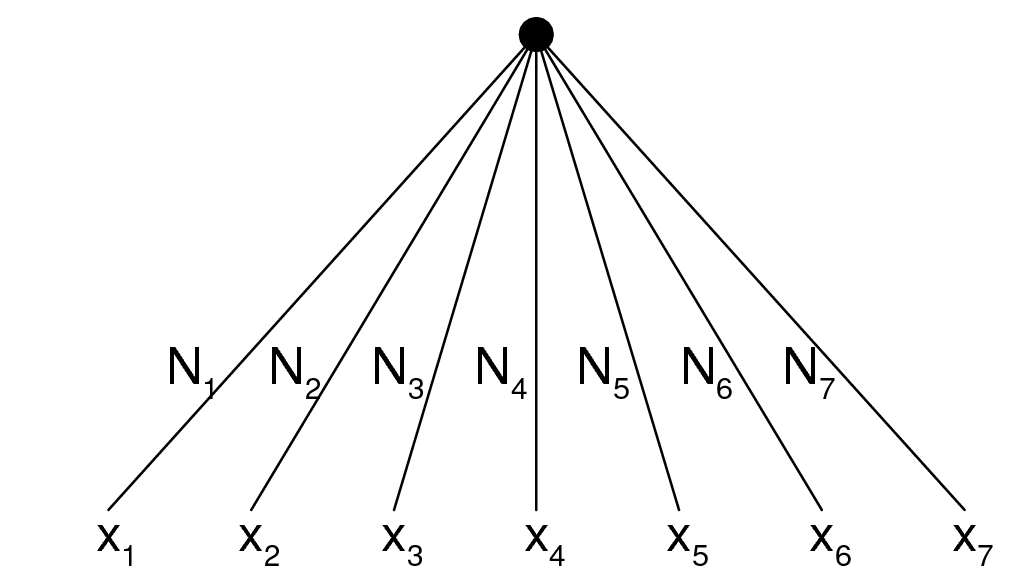
\includegraphics[width=\textwidth]{figures/std_wave}
    \end{subfigure}
    \hfill
    \quad
    \begin{subfigure}[c]{\textwidth}
        \caption{}\label{fig:mctdh_wave}
        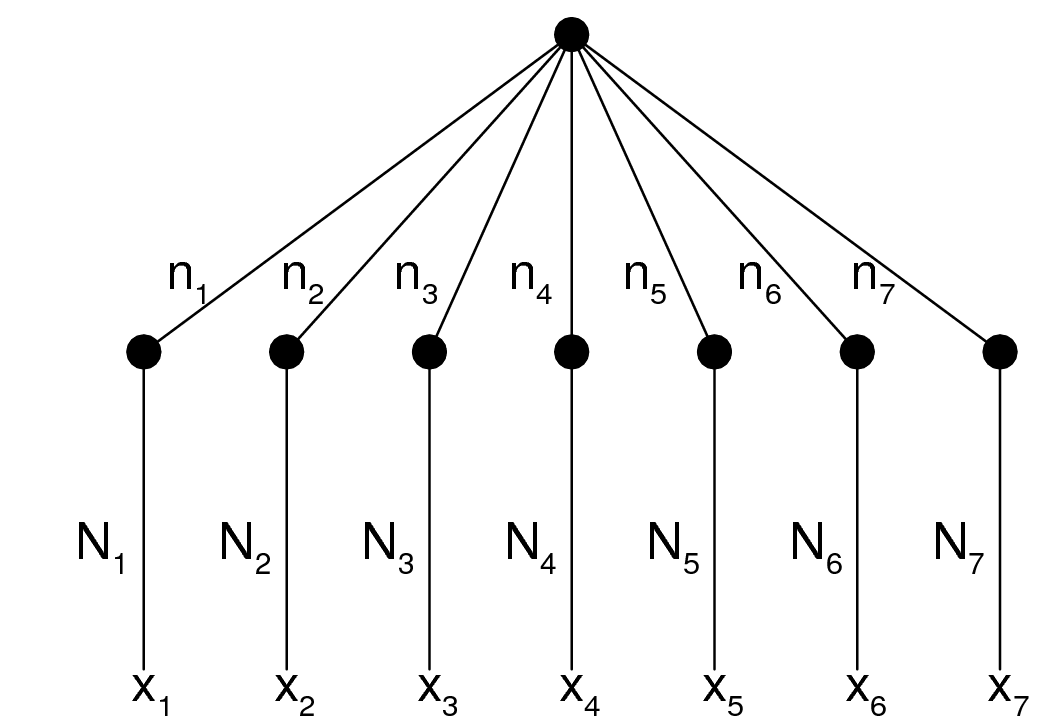
\includegraphics[width=\textwidth]{figures/mctdh_wave1}
    \end{subfigure}
  %  \caption{Left}\label{fig:left}
\end{minipage}
\quad
\begin{minipage}{0.45\textwidth}
    \centering
    \captionsetup[subfigure]{position=top, labelfont=bf,textfont=normalfont,singlelinecheck=off,justification=raggedright}
    \begin{subfigure}{\textwidth}
        \caption{}\label{fig:rightC}
        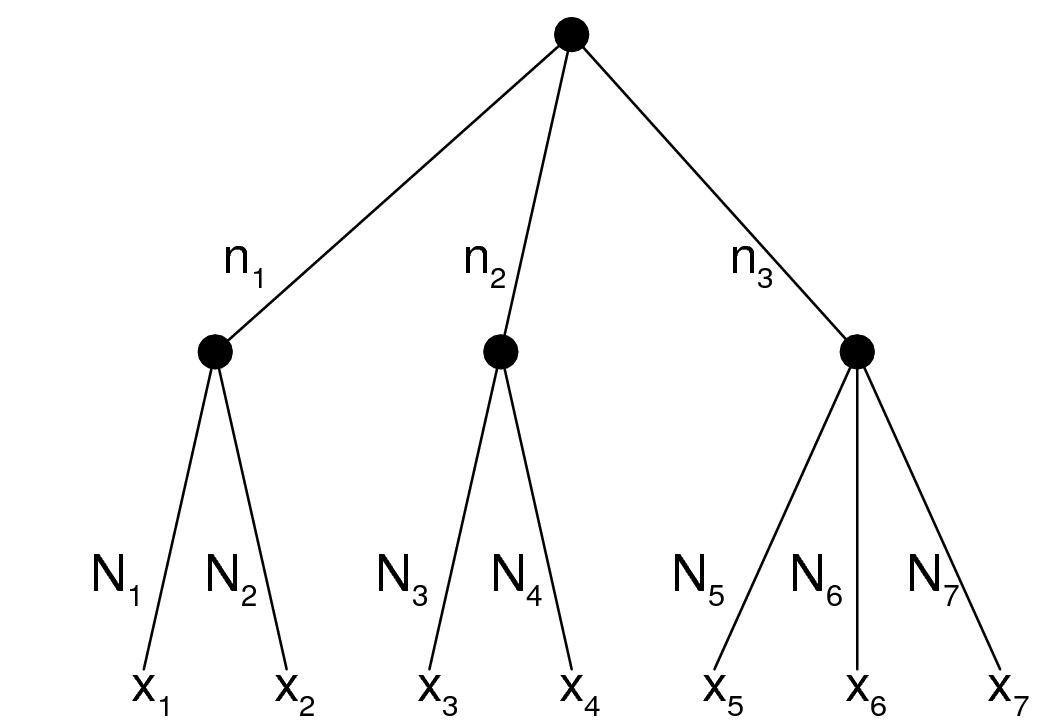
\includegraphics[width=\textwidth]{figures/mctdh_wave2}
    \end{subfigure}
    \quad
    \begin{subfigure}{\textwidth}
        \caption{}\label{fig:multi_mctdh_wave}
        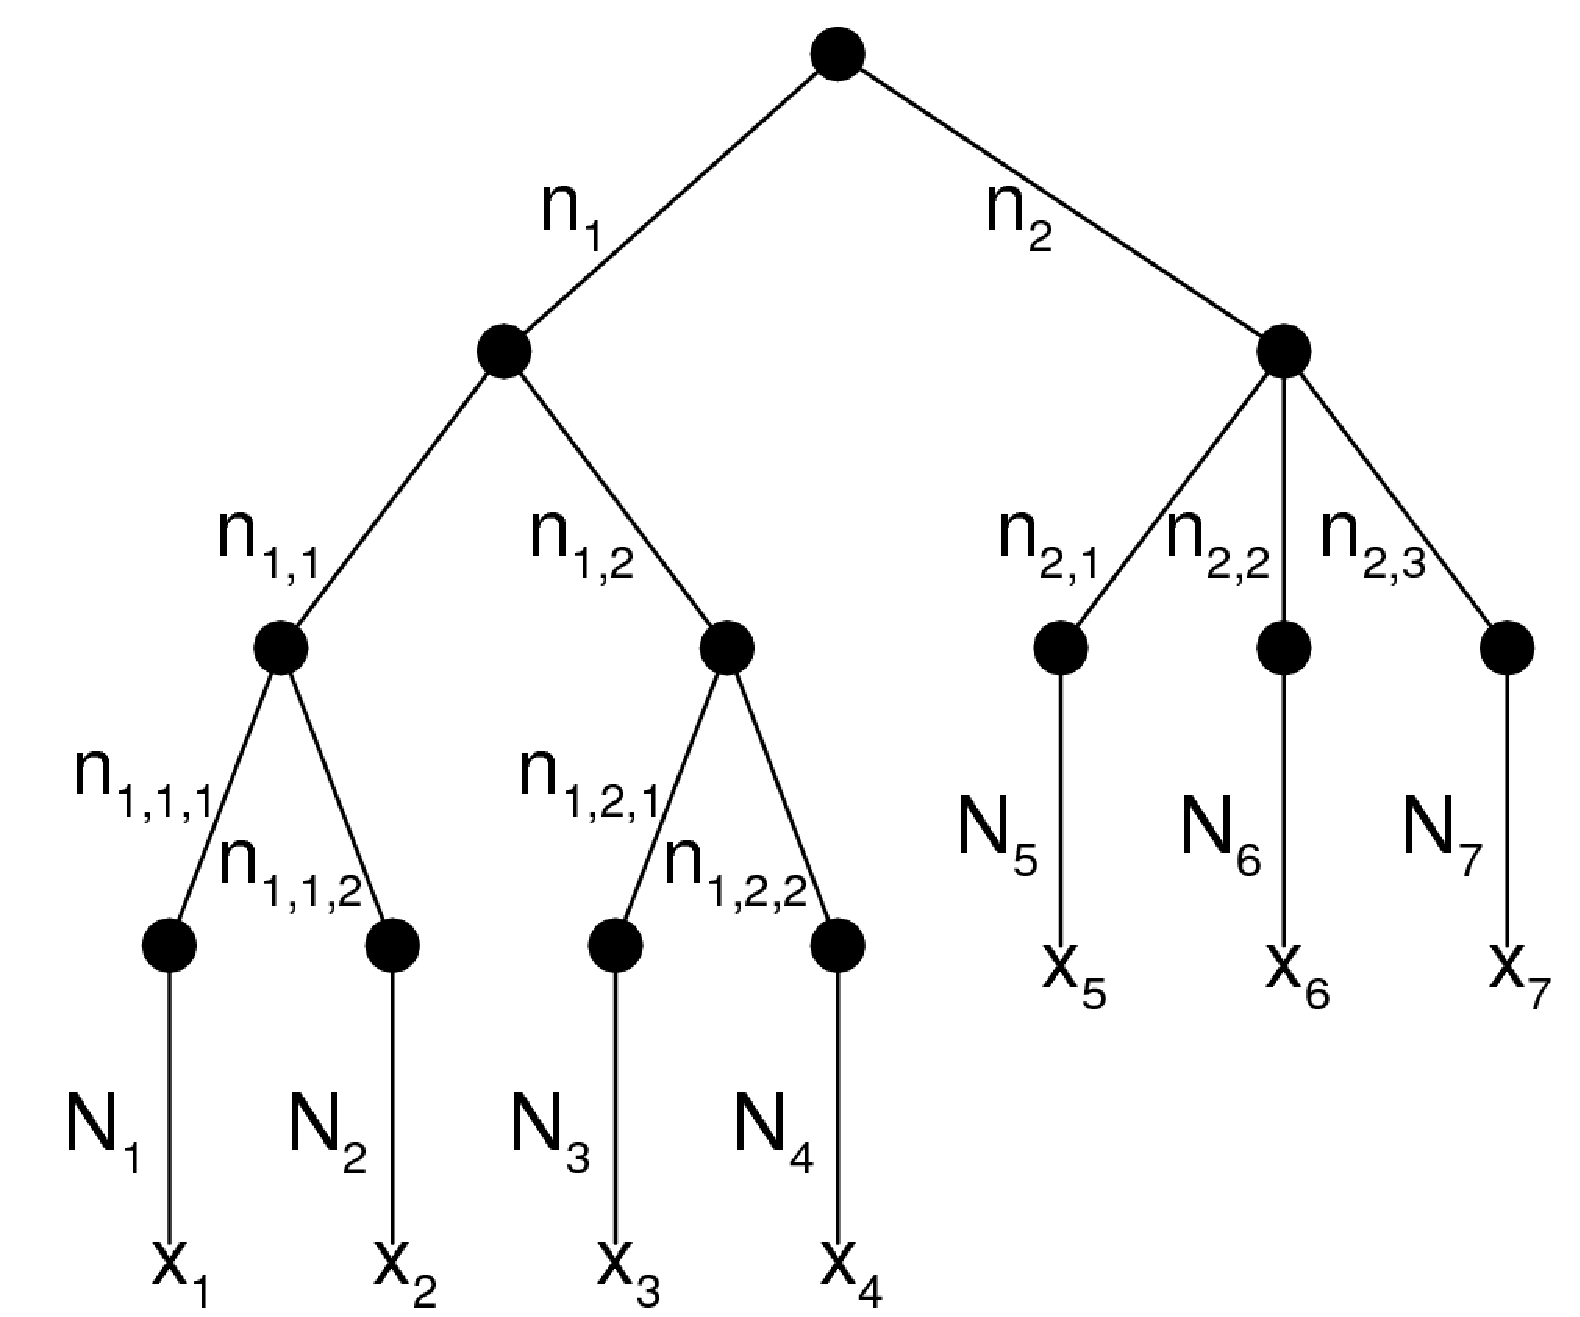
\includegraphics[width=\textwidth]{figures/multi_mctdh_wave}
    \end{subfigure}
%    \caption{right}\label{fig:right}
\end{minipage}
  \caption{Unterschiedliche Darstellung von Wellenfunktionen eines siebendimensionalen Systems. Dargestellt sind: (a) Eine Standard Wellenfunktion,
  (b) eine MCTDH-Wellenfunktion, (c) eine modenkombinierte MCTDH-Wellenfunktion und (d) eine ML-MCTDH-Wellenfunktion.}\label{fig:tree}
\end{figure}









\clearpage
 \subsection{Absorption und Emission}
